\documentclass[11pt]{article}

\usepackage{tikz}
\usepackage{tikz-cd}
\usetikzlibrary{automata}
\usetikzlibrary{arrows}
\usepackage{pgf}
\usepackage{geometry}
\usepackage{float}
\usepackage[parfill]{parskip}
\usepackage[english]{babel}
\usepackage[utf8]{inputenc}
\usepackage{amsmath}
\usepackage{amsfonts}
\usepackage{url}
\usepackage{graphicx}
\usepackage{cite}
\usepackage{hyperref}
\usepackage[colorinlistoftodos]{todonotes}




\title{{\LARGE \sc Dependency Graph Compression}}
\author{}
\date{}

\begin{document}

\maketitle
\thispagestyle{empty}

\section{Introduction}
Current spreadsheets are inefficient for storing large amounts of data with complex formulas. Spreadsheet can be made more efficient by storing these formulas more efficiently.

One aspect of a formula that must be recorded in the spreadsheet is which cells are involved in the calculation and how they relate to, or depend on, one another. We keep track of this information in a dependency table.

\section{Dependency Table}

Each cell or region in the spreadsheet can depend on other cells. For example, if A1 = B1 + C1, then A1’s value depends on B1’s value and C1’s value. We say that B1 and C1 are precedents to A1. Maintaining correct values and calculations is a necessity for spreadsheets. Therefore, any time B1’s or C1’s value is changed, it triggers a recalculation in the spreadsheet; A1’s value must be recalculated using the new value of C1. In fact, any time any cell is updated, the spreadsheet must check to see whether it was a precedent to any other cells and if so recalculate the values of those cells. This creates the need for a structure that efficiently stores these cell relations: the dependency table.

The dependency table can be represented by a directed dependency graph. In the graph, each cell or region of cells, is represented by a node. An edge from node B to node A encodes the cell dependency, namely that B is a precedent of A. This graph only needs to include information regarding cells involved in formulas. A cell that does not depend on anything and is not a precedent to any other cells need not be included in the graph. Furthermore, the dependency graph can only be used to determine which cells need to be recalculated upon an update to a certain cell. It does not store any information regarding the operations performed on the data per the formula’s instructions or how many formulas are in the spreadsheet.

Any time a cell A1 is updated, the spreadsheet must check to see if the cell is a part of the dependency graph in order to ensure that all formulas are correctly executed. More specifically, it must check to see if the A1 is a precedent to any other cells. If no other cells depend on A1, no recalculations are necessary. In terms of the graph, a cell or region that is precedent to no other cells would appear as a node with no outgoing edges. If another cell does depend on A1 (the node does have at least one outgoing edge), then that specific cell value would have to be recalculated. This process would be repeated for any other cells that depend on A1. Similarly, any time a formula is updated, the dependency graph must be updated (nodes and edges added or removed) to reflect the new relationships between cells.

It is entirely possible that a cell is involved in two separate formulas. It is unnecessary for the dependency graph to make the distinction of which nodes and edges in the graph correspond to which formulas, for the dependency graph is only used to determine which cells must be recalculated upon the update of a cell.

The problem with dependency graphs is that, although they do serve a necessary purpose to ensure the accuracy of data, they slow down performance. Any time a cell is updated, the dependency graph must be scanned to see if it contains that cell. The more formulas that a spreadsheet contains and the more cells involved in formulas, the larger the dependency graph. A larger graph leads to a longer amount time required to extract information from the graph. Particularly, if the dependency graph is so large that it cannot fit entirely in main memory, the amount of time to extract information from it can be very lengthy, as it requires disk accesses. Therefore, it is of best interest to limit the size of the dependency graph or find a way to compress the graph. We call this the dependency graph compression problem.

\section{Compressing the Graph}

This compression of the dependency graph can be done in a lossless or lossy manner by combining multiple nodes of the graph. Less nodes (and therefore edges) in the graph requires less space to store the graph.

Consider the example two formulas encoded in the dependency graph: A1 = B1 + C1 and A2 = B1 + C1. The dependency graph containing these two formulas would have four nodes (A1, A2, B1, C1) and four directed edges (B1$\rightarrow$A1, B1$\rightarrow$A2, C1$\rightarrow$A1, and C1$\rightarrow$A2). One way that we could compress this graph is by creating one node to represent the region A1 and A2. The result of this compression would be a graph with three nodes (A1:A1, B1, C1) and two edges (B1$\rightarrow$A1:A2, C1$\rightarrow$A1:A2).

In general, a lossless compression ensures that no information is lost in the new, compressed graph (cell A1 is not recorded in the graph as depending on only B1 when it actually depends on B1 and C1) and no extra information is recorded in the graph (cell A1 is also not recorded in the table as depending on B1, C1, D1, and E1).

When compressing in the lossy manner, we allow extra information to be stored in the dependency graph, for the sake of compression; it is valid to record A1 as depending on B1, C1, D1, and E1. D1 and E1 are false positives, or cells that unnecessarily trigger a recalculation of A1. According to the dependency graph, an update to D1 or E1 requires A1’s value to be recalculated, even though A1’s value will remain the same. 

The total number of false positives in our graph, then, quantifies the amount of extra data that is recorded in the dependency graph, or equivalently, the amount of recalculations that are likely to occur. Now that we have established out metric to distinguish differently compressed graphs, we can compare how effective different compression algorithms are by seeing which fulfills the memory constraint with the lowest number of false positives.

Notice that the dependency graph must only allow for false positives, not false negatives. A false negative occurs when a cell that should trigger a recalculation does not. For example, if A1 is recorded as only depending on B1 (leading to a false negative), then a change to C1’s value would not cause A1’s value to be recalculated. A1’s value is then invalid since A1 = B1 + C1; it does not follow the formula inputted by the user. This is not acceptable behavior from a spreadsheet. 

A false positive causes an extra recalculation, but all of the cell’s values are correct. Therefore, cost of a false positive is the extra time taken for the spreadsheet to respond upon the update of a cell. A small amount of false positives still results in acceptable behavior from the spreadsheet. A large amount of false positives results in very slow performance upon an update to a cell or formula. For example, one correct, and optimal in terms of space, lossy compression of the table would be to encode that every cell depends on every other cell. However, the performance of the spreadsheet would be adversely affected, as an update to any cell would require every other cell to be recalculated.

\section{Optimization}

The task at hand is to find a way to minimize the number of false positives within the dependency table without introducing false negatives within a certain memory constraint. For example, given ten formulas, what is the lowest number of false positives we can have if we only allow there to be eight nodes in the dependency graph. We will analyze algorithms that result in either a lossy or lossless compression, examining which method results in the better performance, in terms of space. We will also test different memory requirements and maximum false positive rates to identify a balance that results in optimal performance.

Given that the nodes of our dependency graph represent cells or regions within a spreadsheet, there are other constraints we must consider when considering this optimization problem.

\begin{enumerate}
    \item \textbf{Shape of region:} If a node does not represent a single cell, there are different types of regions we can consider allowing.
    \begin{enumerate}
    % Is my logic correct here? Please check @Mangesh @Vipul
        \item A region can be required to be rectangular. The benefits of rectangular regions include concise representation (the upper-right corner and the lower-left corner completely define a rectangle) and in spreadsheets, rectangular regions are very common.
        \item A region can be any shape so long as it is contiguous (meaning all cells in the region can reach each other without crossing cells that are not a part of the region). The benefit of contiguous regions is that they allow more flexibility in the compression of the graph without dramatically increasing the number of false positives. However, a non-rectangular region will be more complex to represent and more space to store.
        \item A region can be disjoint. Although more costly to store than contiguous regions, disjoint regions allow the most flexibility in the compression of the graph without dramatically increasing the number of false positives.
    \end{enumerate}
    \item \textbf{Overlap:} We have the options to allow regions to overlap or not overlap. In this case, overlap entails a single cell belonging to more than one region. Again, the benefit of allowing overlaps is more freedom when compressing while keeping the number of false positives low. However, it can cause an increase in time to access data in the graph, as we must determine which regions a cell belongs to before we can return the regions that depend on that cell. These negative performance effects may be able to be mitigated by using an R-tree that behaves by outputting the regions a cell belongs to when given a cell.
\end{enumerate}

\section{NP-Hardness}

Why this problem is NP hard so our greedy solution is acceptable... @Vipul

\section{Greedy Solution}

What Mangesh' code does.

\section{Spreadsheet Applications}

We compressed the dependency graphs from real spreadsheets via the greedy algorithm described above. The following are the results where we restrict the size of the dependency graph to be 30.

Graph 1

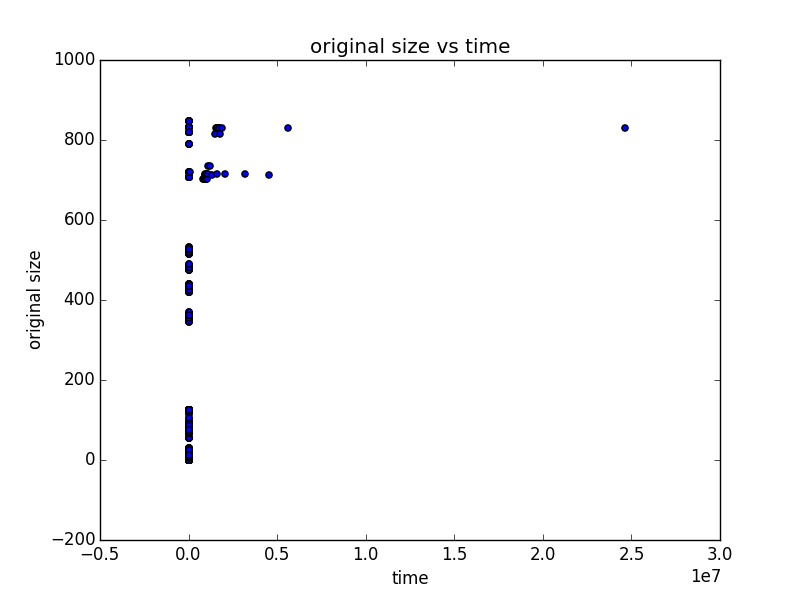
\includegraphics[width=\textwidth]{sizevtime.png}

This graph compares the time it took to compress the graph and the original size of the graph. Clearly, the larger the graph, the more it needs to be compressed, and the longer the compression takes. **can we see a trend here?**

Graph 2

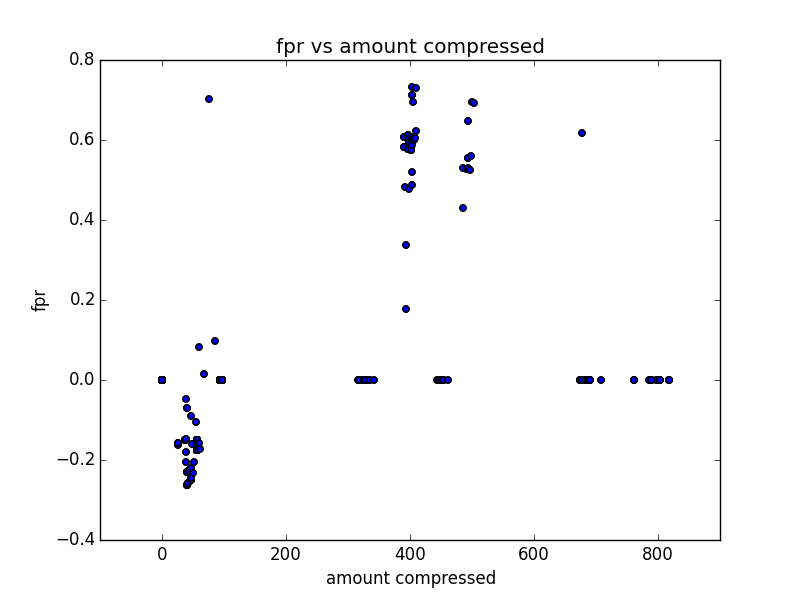
\includegraphics[width=\textwidth]{fprvamountcomp.png}

This graph compares the amount the graph was compressed with the ensuing false positive rate.

Graph 3

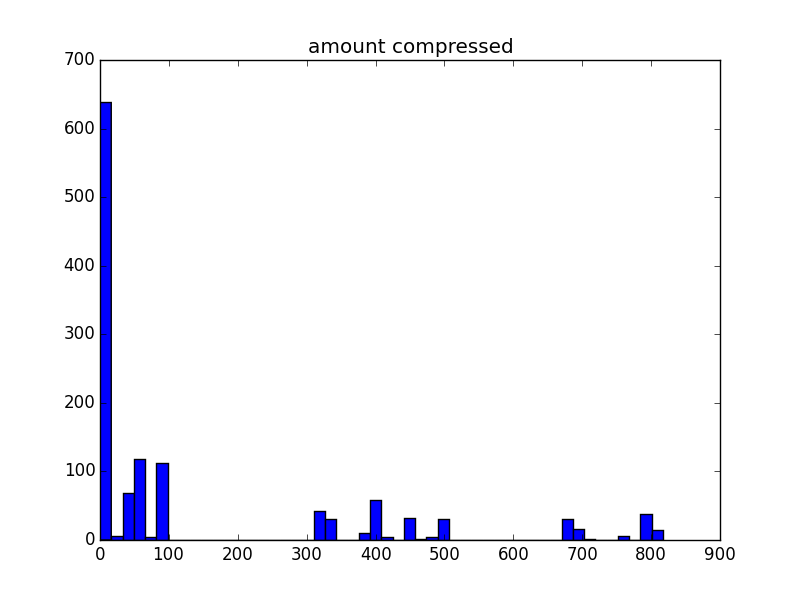
\includegraphics[width=\textwidth]{amountcomp.png}

This is a histogram of the amount the size of the graph decreased due to the compression. As shown, many spreadsheets do not require much compression if any at all. However, there is still a significant number of spreadsheets who were significantly compressed. If we have a memory constraint close to 30, this indicates that many graphs would not be able to fit in main memory and would require many disk accesses.

** TODO: get data about how long it takes to update the compressed graphs, comparing this with false positive rates **
** TODO: change fpr to number of false positives **



%This was back when we said we allowed no overlap and only rectangular regions:
%There are certain restrictions in how we can chose to combine nodes to compress the graph. Each node represents a cell in the spreadsheet or a rectangular region of cells. In either case, merging two nodes will be stored as a rectangular region for ease of representation. Non-rectangular regions are not allowed. To encode a region we simply record the upper-leftmost and lower-rightmost cells. For example, if we were to combine nodes A1 and B2 in the dependency graph, we would remove nodes A1 and B2 from the graph. We would also remove nodes A2 and B1 if they existed to eliminate redundancy of data in the graph. Eliminating this redundancy is necessary because otherwise it would be hard to extract information about which cells a certain cell B2 is precedent to if B2 were represented by multiple different regions in the graph (perhaps one node in the graph is B2, one node is A1:D6, and another is B1:E7). After removing the individual nodes, we add a node A1:B2 which represents the region containing cells A1, A2, B1, and B2. Finally, we add any edges into the graph that had A1, A2, B1, or B2 as an endpoint, except now A1:B2 is the new endpoint. Additionally, all resulting rectangular regions should be disjoint.



\end{document}
